\documentclass[PICOAPC.tex]{subfiles}

\begin{document}

\subsection{Gravitational Waves and Inflation}
\label{sec:inflation}

Measurements of the \ac{CMB} $BB$ angular power spectrum are the only foreseeable way to detect  inflationary gravitational waves. The strength of the signal, quantified by the tensor-to-scalar ratio $r$, is a direct measure of the expansion rate of the Universe during inflation, and together with the Friedmann equation, it reveals the energy scale of inflation. 
%A detection of $r$  ``would be a watershed discovery'', a quote from the 2010 decadal panel report~\citep{blandford2010}. 
%\comred{do you need to explain what BB is?}
PICO will detect primordial gravitational waves at $5\,\sigma$ significance if inflation occurred at an energy scale of at least $5\times 10^{15}\,\rm{GeV}$, or equivalently $r= 5\times 10^{-4}$.  In a widely endorsed community white paper setting targets for measurements of inflationary gravitational waves in the next decade, \citet{Shandera_etal} quote two theoretically motivated $r$ rejection targets: (1) $r < 0.01$, and (2) $r < 0.001$. The second threshold is motivated by the goal of rejecting all inflationary models that naturally explain the observed value of the spectral index %of primordial fluctuations 
$n_{\rm s}$ and having a characteristic scale in the potential that is larger than the Planck scale. Such models are shown in dashed lines in Figure~\ref{fig:nsr}.  
They write "If these thresholds are passed without a detection, most textbook models of inflation will be ruled out; and ...
%while the possibility of an early inflationary phase would still remain viable, 
the data would then force a significant change in our understanding of the primordial Universe." PICO is the only next-decade experiment with the raw sensitivity to reject both targets at high confidence. 
%; see Figure~\ref{fig:nsr}. It is the only next-decade experiment that can detect inflationary models that have $r \geq 5\times 10^{-4}$ at high confidence. 

\begin{figure}[!thb]
\vspace{-.1in}
\hspace{-0.13in}
\parbox{4.4in}{\centerline{
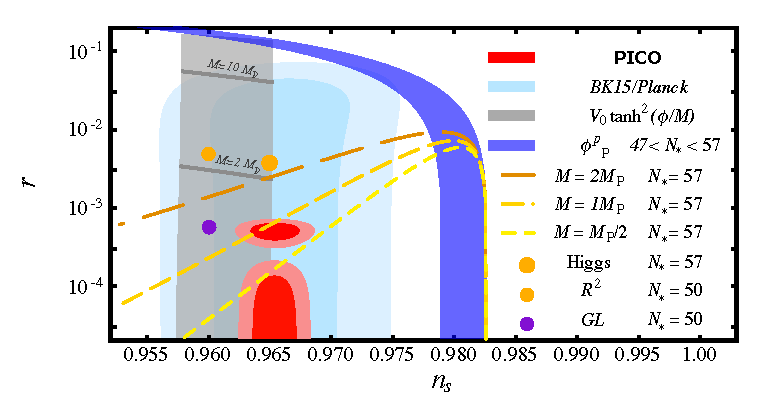
\includegraphics[width=4.5in]{figures/nsrlabeledrp0005_PICOv6.pdf} } }
\parbox{2.1in}{
\caption{\captiontext  PICO will conclusively rule out all Inflation models for which the characteristic scale in the potential is $M_{p}$ or higher, or will detect $r=0.0005$ at $5\, \sigma$ (red 1 and $2\,\sigma$ limits and uncertainty ellipses). Current values of $\sigma_{r}$ are a factor of 100 higher (cyan). 
The locus of classes of models and specific ones are shown with dots, solid, and dashed lines. }
\label{fig:nsr}}
\vspace{-0.16in}
\end{figure}

Uncertainty in the characterization of Galactic foregrounds already limits our ability to constrain $r$. These foregrounds 
are anticipated to be nearly 1000 times stronger than next-decade-targeted inflationary $B$-mode signals at low $\ell$ multipoles. %$\ell=8$. 
`Lensing' $B$-modes, created by gravitational lensing of $E$-modes, are an additional effective foreground for the higher multipoles. With sufficiently high resolution to remove at least 73\% of the lensing effects, and 21 frequency bands to account for foregrounds, no other next-decade experiment is better equipped than PICO to overcome the challenges in in rejecting confusion due to foregrounds.
%robustly finding the faint inflationary signal, or in rejecting confusion due to foregrounds. 

\vspace{-0.06in}

\subsection{Fundamental Particles and Fields} %: Light Relics, Dark Matter, and Neutrinos}
\label{sec:relics_neutrinos}

%\vspace{-0.05in}

$\bullet$ {\bf Light Relics} \hspace{0.1in} The effective number of light relic particle species $\Neff$ gives information about particle species that are predicted to have existed in the early Universe in extensions of the Standard Model. Light particles beyond the three neutrino families contribute a change $\Delta \Neff$ that is a function only of the decoupling temperature of the additional species and the spin of the particle. PICO will provide a constraint $\Delta \Neff < 0.06 \, (95\%)$ and will either detect new particle species, or constrain the lowest decoupling temperature at which any spin 1 particle could have fallen out of equilibrium by a factor of 400 higher than today's constraint~\citep{green_swp}. No next-decade experiment will provide a tighter constraint.   \\ 
%
$\bullet$ {\bf Neutrino Mass} \hspace{0.1in} \label{neutrino_fundamental} The origin, structure, and values of the neutrino masses are among the outstanding questions about the nature of the Standard Model of particle physics.  
Cosmological measurements of $\sum m_\nu$ relate the amplitudes of the matter power spectrum and the primordial fluctuation power spectrum $A_s$.  Both are limited by degeneracies with other parameters. PICO is the only instrument that will self consistently provide three of the four necessary measurement ingredients~\citep{green_swp,dvorkin_swp}. 
In combination with DESI and EUCLID data, PICO will give $\sigma(\sum m_\nu) = 14$ meV, giving a $4\,\sigma$ detection of the minimum sum of 58~meV. PICO will measure  $\sum m_\nu$ in two additional ways, which will give equivalent constraints. \\
%
$\bullet$ {\bf Dark Matter} \hspace{0.1in} \ac{CMB} experiments are effective in constraining dark matter candidates in the lower mass range, which is not available for terrestrial direct detection experiments~\citep{Slatyer2009,Galli2009,Huetsi2009,Huetsi2011,Madhavacheril:2013cna,Green:2018pmd}. 
For a spin- and velocity-independent contact interaction between dark matter and protons PICO will improve upon \planck 's dark matter cross-section constraints by a factor of 25 over a broad range of candidate dark matter masses. If 2\% of the total dark matter content is made of axions in the mass range $10^{-30} < m_{a} < 10^{-26}$, PICO will detect this species at between $7$ and $13\,\sigma$.  These constraints are stronger than other proposed next-decade CMB experiments~\citep{gluscevic_swp}. \\
%
$\bullet$ {\bf Primordial Magnetic Fields (PMFs)} \hspace{0.1in} PICO is the only experiment that can probe PMFs as weak as 0.1~nG ($1\,\sigma$).  Detection of PMFs would be a major discovery because it would signal new physics beyond the Standard Model, discriminate among different theories of the early Universe, and explain the puzzling $1 - 10~\mu$G fields observed in galaxies.  Or it could conclusively rule out a purely primordial (i.e., no-dynamo-driven) origin of the largest galactic magnetic fields~\citep{Widrow:2002ud,Widrow:2011hs,Athreya:1998,Grasso:2000wj,Vachaspati:1991nm,Turner:1987bw,Ratra:1991bn,DiazGil:2007dy,Barnaby:2012tk,Long:2013tha,Durrer:2013pga}. \\
%
$\bullet$ {\bf Cosmic Birefringence} \hspace{0.1in}
A number of well-motivated extensions of the Standard Model involve fields with parity-violating coupling~\citep{Freese:1990rb,Frieman:1995pm,Carroll:1998zi,Kaloper:2005aj,2008PhRvL.101n1101C,Gluscevic:2010vv}. Their presence may cause cosmic birefringence -- a rotation of the polarization of an electromagnetic wave as it propagates across cosmological distances~\cite{Harari:1992ea,Carroll:1989vb,Carroll:1998zi}. PICO's constraints on cosmic birefringence are more stringent than any other next-decade experiment~\cite{pogosian_2019}. 


\end{document}

%$\bullet$ {\bf Primordial Magnetic Fields} \hspace{0.1in} One of the long-standing puzzles in astrophysics is the origin of observed 1--10~$\mu$G galactic magnetic fields~\citep{Widrow:2002ud}. Producing such fields through a dynamo mechanism requires a primordial seed field~\citep{Widrow:2011hs}. Moreover, $\mu$G-strength fields have been observed in proto-galaxies that are too young to have gone through the number of revolutions necessary for the dynamo to work~\citep{Athreya:1998}. A 0.1~nG primordial magnetic field (PMF), present at the time of galaxy formation, could provide the seed or even eliminate the need for the dynamo altogether~\citep{Grasso:2000wj}. 
%%Specifically, a 0.1~nG field in the intergalactic plasma would be adiabatically compressed in the collapse to form a $\sim$1~$\mu$G galactic field~\citep{Grasso:2000wj}.
%PMFs could have been generated in the aftermath of phase transitions in the early Universe~\citep{Vachaspati:1991nm}, during inflation~\cite{Turner:1987bw,Ratra:1991bn}, or at the end of inflation~\cite{DiazGil:2007dy}. 
%A detection of PMFs with the CMB would be a major discovery because it would signal new physics beyond the Standard Model, and discriminate among different theories of the early Universe~\cite{Barnaby:2012tk,Long:2013tha,Durrer:2013pga}. PICO will probe PMFs as weak as 0.1~nG ($1\sigma$), a precision not attainable by any next-decade experiment, and can thus conclusively rule out the purely primordial (i.e., no-dynamo driven) origin of the largest galactic magnetic fields. \\

%$\bullet$ {\bf Cosmic Birefringence} \hspace{0.1in}
%A number of well-motivated extensions of the Standard Model involve fields with parity-violating coupling~\citep{Freese:1990rb,Frieman:1995pm,Carroll:1998zi,Kaloper:2005aj,Carroll:1998zi,2008PhRvL.101n1101C,Gluscevic:2010vv}. Their presence may cause cosmic birefringence -- a rotation of the polarization of an electromagnetic wave as it propagates across cosmological distances~\cite{Harari:1992ea,Carroll:1989vb,Carroll:1998zi}. PICO's constraints on cosmic birefringence are more stringent than any other next-decade experiment~\cite{pogosian_2019}. 


